

\section{The Reshape package}

|reshape2| is an R package for restructuring, transforming, and summarizing multivariate data sets. |reshape2| was written by Hadley Wickham, a statistician at Rice University, who is also the author of ggplot.  In this chapter we'll just scratch the surface of this package; for a more detailed overview see the documentation available on reshape web page -- \href{http://had.co.nz/reshape/}{reshape}. Install the |reshape2| package before proceeding.

The |reshape2| package allows us to restructure and aggregate data more easily than the built-in R functions.  There are two primary functions associated with the package -- |melt()| and |cast()|.  We use |melt()| to restructure a data frame or list into a generic structure that can then be |cast()| into the form we want.


\subsubsection{melt}

Import the |reshape2| package with |library(reshape2)| and read the docs for the |melt()| function.  |melt()| needs at least three arguments: 1) a data frame or list, 2) a vector specifying which columns to treat as `identification variables' (|id.vars|), and 3) a vector specifying which columns to use as `measured variables' (|measured.vars|).  ID variables are typically the fixed variables that represent aspects of the experimental design while measured variables represent the variables that were measured on each unit of interest.  If |id.vars| and |measured.vars| aren't specified, the |melt()| function will try and infer the |id.vars| based on those columns that are factors, and treat the remaining variables as |measured.vars|.  If only |id.vars| is specified, the remaining variables will be treated as |meaured.vars|.

Let's create a simple data set that we can use to explore |melt()| and |cast()| functions.
%
\begin{R}
> group1 <- c(rep("A", 9), rep("B",9))
> group2 <- rep(c("1","2","3"),6)
> data1 <- c(rnorm(9,mean=0), rnorm(9,mean=1))
> data2 <- as.vector(t(mapply(rnorm, n = c(3,3,3,3,3,3), mean = c(0,1,3))))
> test.data <- data.frame(species=as.factor(group1), 
                          treatment=as.factor(group2), 
                          v1=data1, v2=data2)
> test.data
   species treatment          v1          v2
1        A         1  0.75357665 -1.83527194
2        A         2  0.40335481  1.22663973
3        A         3  1.18084161  4.47310654
4        A         1 -0.18393749 -1.61953719
5        A         2 -0.85328571  2.75230914
6        A         3  0.99141392  3.39575430
7        A         1 -1.12026845 -0.61442409
8        A         2 -0.01716075  2.08970130
9        A         3 -1.84389967  2.08822132
10       B         1 -0.30507545 -0.01171179
11       B         2  0.54634457 -0.31179921
12       B         3  2.38310469  4.02453740
13       B         1  0.95729799  0.14273026
14       B         2  3.14992630  1.01718329
15       B         3  1.28400301  2.16849192
16       B         1  0.94616082 -0.26436515
17       B         2  1.19047574  0.58964302
18       B         3  0.35085358  2.46990925
\end{R}
%

Let's apply |melt()|, specifying the `species' and `treatment' columns as the |id.vars|.
%
\begin{R}
> melt.test <- melt(test.data, id.vars = c("species","treatment"))
> melt.test
   species treatment variable       value
1        A         1       v1  0.75357665
2        A         2       v1  0.40335481
3        A         3       v1  1.18084161
....
13       B         1       v1  0.95729799
14       B         2       v1  3.14992630
15       B         3       v1  1.28400301
....
19       A         1       v2  1.91999253
20       A         2       v2  1.76509214
21       A         3       v2  3.33803728
....
28       B         1       v2  3.63924057
29       B         2       v2  1.81988816
30       B         3       v2  2.00163369
\end{R}
%
Examining the melted data set, you'll see that the columns representing the measured variables have been collapsed into a single new column called `value'.  There is also another column called `variable' which specifies which of the measured variables the items in `value' came from.

\subsubsection{cast}

Having melted our data set, we can then use the |cast()| function to reshape and aggregate the data into the form we desire.  Read the docs for |cast()|.  Note that the |cast()| function is actually caleld as |dcast()| or |acast()| depending on whether you want the function to return a data frame or a vector or array. Minimally, |cast()| takes: 1) a melted data set,  2) a formula specifying how to shape the melted data; and 3) a function to apply to any aggregates that are specified for the cast formula. These are most easily illustrated by example, as shown below.

In the first example we're going to aggregate the measurements of each variable for each species and calculate the species mean.  Notice the form of the formula -- |species ~ variable|.
%
\begin{R}
> recast.test <- dcast(melt.test, species ~ variable, mean)
> recast.test
  species          v1       v2
1       A -0.07659612 1.328500
2       B  1.16701014 1.091624
\end{R}

In the second example, we want to aggregate across species \emph{and} experimental treatments.  The resulting values in the table show the per-species-per-treatment means.
\begin{R}
> recast.test <- dcast(melt.test, species + treatment ~ variable, mean) 
> recast.test
  species treatment         v1          v2
1       A         1 -0.1835431 -1.35641107
2       A         2 -0.1556972  2.02288339
3       A         3  0.1094520  3.31902738
4       B         1  0.5327945 -0.04444889
5       B         2  1.6289155  0.43167570
6       B         3  1.3393204  2.88764619   
\end{R}



\subsubsection{Yeast NanoString Dataset}

To illustrate the use of the |reshape2| package in conjunction with |ggplot2| we will use another gene expression data set my lab has generated.  This data set includes time series expression measurements on 192 genes, collected on each of four different yeast strains grown under two different media conditions. Each treatment (time point, media condition, strain) was replicated three times.  The expression platform used for this study is a technology called \href{http://www.nanostring.com/}{NanoString}.

Download the data set |yeast-timeseries.csv| from the course wiki. The data file is a plain text file that uses the "comma separated values" format. Use the |read.csv| function to read this data into R.
%
\begin{R}
> yeast.time <- read.csv('yeast-timeseries.csv')
> dim(yeast.time)
[1] 108 196
> names(yeast.time)
  [1] "sample.id"  "media"      "strain"     "time.pt"    "replicate"  "ACE2"      
  [7] "ACT1"       "ADR1"       "AGA2"       "AMN1"       "ASG7"       "ASH1" 
...
\end{R}

We want to treat |sample.id|, |media|, |strain|, and |replicate| as factors.   Of these, |strain| isn't the only variable that is not automatically treated as a factor, because the strain names are numbers. Let's change that as follow:
%
\begin{R}
> yeast.time$strain <- as.factor(yeast.time$strain)
\end{R}
%

Now let's melt the data set:
%
\begin{R}
> yeast.melt <- melt(yeast.time, 
        id.vars = c("sample.id","strain","media","replicate","time.pt"))
> dim(yeast.melt)
[1] 20628     7
\end{R}
%
For our example we'll aggregate across species, media conditions, and time points and calculate the respective means.  Below is the appropriate |dcast()| call and the first few rows and columns of the reshaped matrix.
%
\begin{R}
> yeast.cast <- dcast(yeast.melt, strain + media + time.pt ~ variable, mean)
> dim(yeast.cast)
[1]  36 194
> yeast.cast[1:10,1:5]
   strain media time.pt      ACE2      ACT1
1     144 YEPLD      24 479.99997 95666.580
2     144 YEPLD      48 198.66663 50803.660
3     144 YEPLD      72 119.83327 25328.243
4     144 YEPLD      96  53.19444 18782.137
5     144   YPD       0 470.88887 92196.660
6     144   YPD      24 481.80550 95400.580
7     144   YPD      48 122.55554 40365.830
8     144   YPD      72  53.55555 18454.160
9     144   YPD      96  53.33333  8317.555
10    497 YEPLD      24 510.72220 95666.580
\end{R}

Now let's generate a time series plot for the first gene in the data set, ACE2:
\begin{R}
> ggplot(subset(yeast.cast, media == 'YPD'), 
        aes(x=time.pt, y=ACE2, col=strain)) + geom_line() + geom_point()
\end{R}
%
Notice the use of the |subset()| function to focus specifically on the YPD media treatment.  However, it would be much more useful to be able to compare the two media treatments, YPD and YEPLD, side by side.  To do so we can use what ggplot calls a `facet'.  A facet  specifies one or more variables to condition against.  So if we treate the variable |media| as a facet, we will generate a set of plots that differ only by media type.  Here's how to do this simply with the |facet_wrap()| function from ggplot:
\begin{R}
> ggplot(yeast.cast, aes(x=time.pt, y=ACE2, col=strain)) + geom_line() + geom_point() + facet_wrap(facets=c('media'))
\end{R}
%
Your plot should resemble Fig.~\ref{fig:yeasttime}.
\begin{figure}[htbp]
\centering
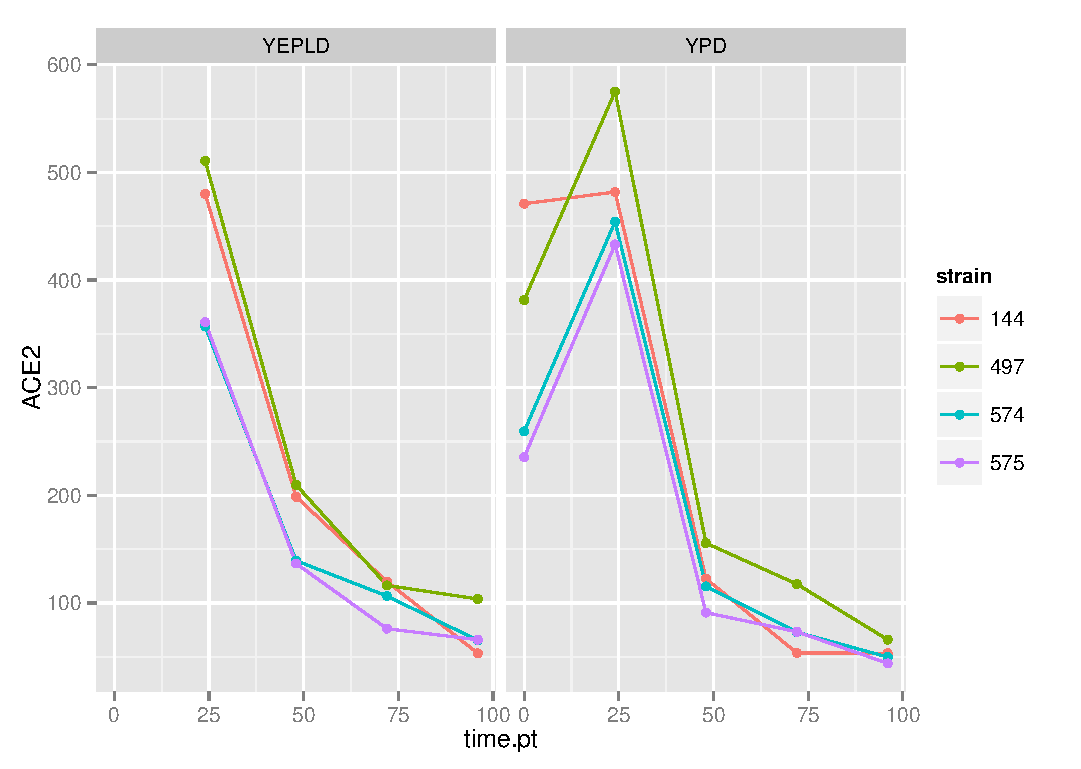
\includegraphics[width=0.7\columnwidth]{./figures/hands-on3/yeast-timeseries-plot.pdf}
\caption{Gene expression time series for four yeast strains generated, grown in two different media conditions.\label{fig:yeasttime}}
\end{figure}
